\documentclass{article}
\usepackage{amsmath}
\usepackage{amssymb}
\usepackage{bm}
\usepackage{graphicx}
\usepackage{epstopdf}
\DeclareGraphicsRule{.tif}{png}{.png}{`convert #1 `basename #1 .tif`.png}
\usepackage{color}
\pagestyle{plain}
%\pagestyle{empty}
\textheight 9 true in
\textwidth 6.5 true in
\hoffset -.75 true in
\voffset -.75 true in
 
\mathsurround=2pt  \parskip=2pt
\def\crv{\cr\noalign{\vskip7pt}} 
\def\a{\alpha } \def\b{\beta } \def\d{\delta } \def\D{\Delta } \def\e{\epsilon }
\def\g{\gamma } \def\G{\Gamma} \def\k{\kappa} \def\l{\lambda } \def\L{\Lambda }
\def\th{\theta } \def\Th{\Theta} \def\r{\rho} \def\o{\omega} \def\O{\Omega}
\def\ve{\varepsilon} 

\def\sA{{\cal A}} \def\sB{{\cal B}} \def\sC{{\cal C}} \def\sI{{\cal I}}
\def\sR{{\cal R}} \def\sF{{\cal F}} \def\sG{{\cal G}} \def\sM{{\cal M}}
\def\sT{{\cal T}} \def\sH{{\cal H}} \def\sD{{\cal D}} \def\sW{{\cal W}}
\def\sL{{\cal L}} \def\sP{{\cal P}} \def\s{\sigma } \def\S{\Sigma}
\def\sU{{\cal U}} \def\sV{{\cal V}} \def\sY{{\cal Y}}

\def\gm{\gamma -1}
\def\summ{\sum_{j=1}^4}

\def\bb{{\bm b}} \def\yb{{\bm y}}
\def\ub{{\bm u}}  \def\xb{{\bm x}} \def\vb{{\bm v}} \def\wb{{\bm w}}
\def\omegab{{\bm \omega}} \def\rb{{\bm r}} \def\ib{{\bm i}} \def\jb{{\bm j}}
\def\lb{{\bm l}} \def\kb{{\bm k}} \def\Ab{{\bm A}} \def\fb{{\bm f}} \def\Ub{{\bm U}}
\def\Fb{{\bm F}} \def\nb{{\bm n}} \def\Db{{\bm D}} \def\eb{{\bm e}}
\def\gb{{\bm g}}  \def\Gb{{\bm G}} \def\hb{{\bm h}} \def\Yb{{\bm Y}} \def\Rb{{\bm R}} 
\def\Tb{{\bm T}}

\def\As1{{\bf {\cal A}}_1}\def\DO{{\cal D}_0} \def\UO{{\cal U}_0}
\def\ie{{\it{i.e.}}}

\def\ubbar{{\bf {\bar{u}}}} \def\sbar{{\bar{\sigma }}} \def\ubar{{\bar{u}}}  
\def\abar{{\bar{a}}} \def\vbar{{\bar{v}}}  \def\rbar{{\bar{\rho}}}
\def\pbar{{\bar{p}}} \def\ebar{{\bar{e}}} \def\Tbar{{\bar{T}}}
\def\bbar{{\bar{\beta}}} \def\Mbar{{\bar{M}}}  \def \sMbar{{\bar{\cal M}}}
\def\Ebar{{\bar{E}}} \def\sMbar{{\bar{\cal M}}}
\def\sPbar{{\bar{\cal P}}} \def\xbar{{\bar{x}}}

\newcommand{\pdv}[2]{\frac{\partial#1}{\partial#2}}
\newcommand{\dv}[2]{\frac{d#1}{d#2}}
\newcommand{\ord}[2]{#1^{(#2)}}
\newcommand{\vct}[1]{\vec{#1}}

 \newcommand{\bc}{\begin{center}}
 \newcommand{\ec}{\end{center}}
 
 \newcommand{\bq}{\begin{equation}}
 \newcommand{\eq}{\end{equation}}
 
 \newcommand{\beqs}{\begin{eqnarray}}
 \newcommand{\eeqs}{\end{eqnarray}}
 
 \newcommand{\beqa}{\begin{eqnarray*}}
 \newcommand{\eeqa}{\end{eqnarray*}}
 
 \newcommand{\ol}{\overline}
 \newcommand{\ul}{\underline}
 
 \newcommand{\dint}{{\int \!\! \int \!\!}}
 \newcommand{\tint}{{\int \!\! \int \!\! \int \!\!}}
 
 \newcommand{\bfig}{\begin{figure}}
 \newcommand{\efig}{\end{figure}}
 
 \newcommand{\cen}{\centering}
 \newcommand{\n}{\noindent}
 
 \newcommand{\btab}{\begin{table}}
 \newcommand{\etab}{\end{table}}
 
 \newcommand{\btbl}{\begin{tabular}}
 \newcommand{\etbl}{\end{tabular}}
 
 \newcommand{\bdes}{\begin{description}}
 \newcommand{\edes}{\end{description}}
 
 \newcommand{\benum}{\begin{enumerate}}
 \newcommand{\eenum}{\end{enumerate}}
 
 \newcommand{\bite}{\begin{itemize}}
 \newcommand{\eite}{\end{itemize}}
 
 \newcommand{\cle}{\clearpage}
 \newcommand{\npg}{\newpage}
 
 \newcommand{\bss}{\begin{singlespace}}
 \newcommand{\ess}{\end{singlespace}}
 
 \newcommand{\bhalf}{\begin{onehalfspace}}
 \newcommand{\ehalf}{\end{onehalfspace}}
 
 \newcommand{\bds}{\begin{doublespace}}
 \newcommand{\eds}{\end{doublespace}}
 
 \newcommand{\eps}{\mbox{$\epsilon$}} 
 \newcommand{\stilde}{\mbox{$\tilde s$}} 
 \newcommand{\shat}{\mbox{$\hat s$}} 

 \newcommand{\blue}{\color{blue}}
 \newcommand{\red}{\color{red}}
 \newcommand{\magenta}{\color{magenta}}
 \newcommand{\green}{\color{green}}
 \newcommand{\nc}{\normalcolor}




\pagestyle{empty}
\begin{document}

\begin{center}
\large{ MATH-6620 \hspace{1in}  PERTURBATION METHODS \hspace{1in}SPRING 2016\\ Homework-5 \\ Assigned Tuesday April 5, 2016 \\ Due Monday April 18, 2016.}\end{center}

\bigskip
\bc {\bf PROBLEMS} \ec

\benum

% Problem 1
\item Use the multiple-scales technique, with $t$ as the fast time and $\tau = \e t$ the slow time, to compute the leading-order approximation, valid for long time, to the problem
%
\begin{equation*}
\frac{d^2u}{dt^2} + u + \e \left( u-a\frac{du}{dt} \right)^3 = 0, \;\; t>0; \quad u(0)=1,\;\frac{du}{dt}(0)=0.
\end{equation*}
%
Here the constant $a>0$ is independent of $\e.$  Explain what happens to your solution when $a<0.$\\

Solution:\\

We begin by setting $\tau=\e$ and $u(t;\e)=U(t,\tau;\e)$ to transform the ODE into the PDE
$$U_{tt}+U+2\e U_{t\tau}+\e(U-a[U_t+\e U_\tau])^3+\e^2U_{\tau\tau}=0,\;\;U(0,0)=1,\;\;U_t(0,0)+\e U_\tau(0,0)=0.$$
We then let $U(t,\tau;\e)\sim U_0(t,\tau)+\e U_1(t,\tau)$ to get the resulting $O(1)$ and $O(\e)$ equations. The $O(1)$ equation is as follows,
$$\e^0:\;\;U_{0tt}+U_0=0,\;\;U_0(0,0)=1,\;\;U_{0t}(0,0)=0,$$
with solution
$$U_0(t,\tau)=f_0(\tau)\sin(t+\phi(\tau)),\;\;f_0(0)=1,\;\;\phi(0)=\frac{\pi}{2}.$$
We then inspect the $O(\e)$ equation to determine $f_0$ and $\phi$.
$$\e^1:\;\;U_{1tt}+U_1=-(U_0-aU_{0t})^3-2U_{0t\tau}.$$
When we substitute in our previously determined values for $U_0$, the right hand side of the equation becomes
$$\text{RHS}=-\frac{f_0^3}{4}\left[-3a\cos(t+\phi)-a^3\cos(3t+3\phi)+3a^2\sin(t+\phi)+3a^2\sin(2t+3\phi)-3a\cos(t+\phi)\right.$$
$$\left.+3a\cos(3t+3\phi)+3\sin(t+\phi)-\sin(3t+3\phi)\right]-2f_0'\cos(t+\phi)+2f_0\phi'\sin(t+\phi).$$
In order to remove secularity from the $O(\e)$ PDE, the coefficients on $\cos(t+\phi)$ and $\sin(t+\phi)$ must be set to 0. Thus we have two ODE's:
$$f_0'=f_0^3\frac{3a}{8}(a^2+1),\;\;f_0(0)=1$$
$$\phi'=\frac{3}{8}f_0^2(a^2+1),\;\;\phi(0)=\frac{\pi}{2}.$$
The solution to the first equation is
$$f_0(\tau)=\frac{2}{\sqrt{4-3a(a^2+1)\tau}},$$
which allows us to find the solution of the second equation,
$$\phi(\tau)=\frac{\pi}{2}+\frac{1}{2a}\log\left|\frac{4}{3a^3\tau+3a\tau-4}\right|.$$
Thus our leading order approximation is
$$U_0(t,\tau)=\frac{2}{\sqrt{4-3a(a^2+1)\tau}}\cos\left[t+\frac{1}{2a}\log\left|\frac{4}{3a^3\tau+3a\tau-4}\right|\right].$$
If we rewrite this in terms of $t$ only, we get
$$u_0(t)=\frac{2}{\sqrt{4-3a(a^2+1)\e t}}\cos\left[t+\frac{1}{2a}\log\left|\frac{4}{3a^3\e t+3a\e t-4}\right|\right].$$
We can see in the form of the solution that there is going to be a vertical asymptote when
$$\frac{4}{3 \e a(a^2+1)}=t$$
if $a$ is positive. However, if $a$ is negative, our solution will be oscillatory and slowly decaying. Plots of the solution for $a=-1$ and $a=1$ are below.

\begin{figure}[h]
  \centering
  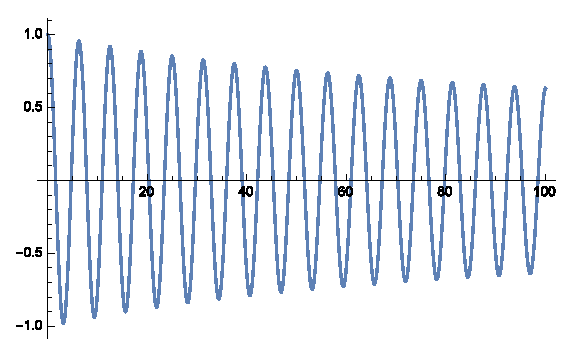
\includegraphics[width=3in]{pertsHW5no1img1.eps}
  \caption{Plot of $u_0$ with $a=-1$ and $\e=.01$. }
\end{figure}
\begin{figure}
  \centering
  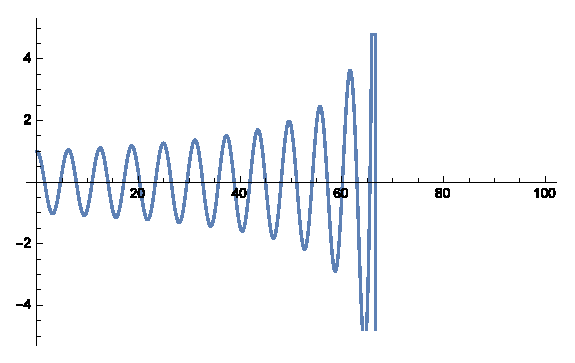
\includegraphics[width=3in]{pertsHW5no1img2.eps}
  \caption{Plot of $u_0$ with $a=1$ and $\e=.01$.}
\end{figure}

\pagebreak

% Problem 2
\item Use the multiple-scales technique, with $t$ as the fast time and $\tau = \e t$ the slow time, to compute the leading-order approximation, valid for long time, to the problem
%
\begin{equation*}
\frac{d^2u}{dt^2} + \{1+\e \sin(\e t)\} u + \e \left(\frac{du}{dt} \right)^3 = 0, \;\; t>0; \quad u(0)=1,\;\frac{du}{dt}(0)=0.
\end{equation*}

Solution:\\

We let $\tau=\e t$ and $u(t;\e)=U(t,\tau;\e)$ to transform the ODE above into the PDE
$$U_{tt}+(1+\e\sin(\tau))U+2\e U_{t\tau}+\e(U_t+\e U_{\tau})^3=0,\;\;U(0,0)=1,\;\;U_t(0,0)+\e U_{\tau}(0,0)=0.$$
Next we let $U(t,\tau;\e)\sim U_0(t,\tau)+\e U_1(t,\tau)$ to get the two-leading order approximation equations. The $O(1)$ equation is
$$U_{0tt}+U_0=0,\;\; U_0(0,0)=1,\;\;U_{0t}(0,0)=0,$$
with solution
$$U_0(t,\tau)=f_0(\tau)\sin(t+\phi(\tau)),\;\; \phi(0)=\frac{\pi}{2},\;\;f_0(0)=1.$$
The $O(\e)$ equation is then
$$U_{1tt}+U_1=-2U_{0t\tau}-\sin(\tau)U_0-U_{0t}^3.$$
The right hand side of this equation, once $U_0$ is substituted in gives us
$$\text{RHS}=-2[f_0'\cos(t+\phi)-f_0\phi'\sin(t+\phi)]-f_0\sin(\tau)\sin(t+\phi)-\frac{f_0^3}{4}(3\cos(t+\phi)+\cos(3t+3\phi)).$$
Elimination of secularity demands
$$f_0'+\frac{3f_0^3}{8}=0,\;\;f_0(0)=1\;\;\implies f_0(\tau)=\frac{2}{\sqrt{4+3\tau}}$$
$$\phi'=\frac{\sin(\tau)}{2},\;\; \phi(0)=\frac{\pi}{2}\;\;\implies \phi(\tau)=\frac{\pi+1}{2}-\frac{\cos(\tau)}{2}.$$
This then gives the leading-order approximation
$$U_0(t,\tau)=\frac{2}{\sqrt{4+\tau}}\cos\left[t+\frac{1}{2}-\frac{\cos(\tau)}{2}\right].$$
If we write this in the original variables and let $u_0\sim u$, we get
$$u_0(t)=\frac{2}{\sqrt{4+3\e t}}\cos\left[t+\frac{1}{2}-\frac{\cos(\e t)}{2}\right].$$
As the change in frequency is $O(\e^2)$, we can get an even simpler leading-order approximation
$$u_0=\frac{2}{\sqrt{4+3\e t}}\cos(t).$$


% Problem 3
\item Consider the weakly nonlinear equation
\begin{equation*}
u_{tt} - u_{xx} + u + \e u^2 = 0, \quad |x|<\infty, \; t>0.
\end{equation*}
Note that we considered a similar equation in class but with a cubic nonlinearity.  Find a multi-scale expansion for the right-running wave that removes the secular term coming from the nonlinearity.  Note also that the scales needed to remove the secular term in this problem are different from those needed for the problem with cubic nonlinearity.  Comment on what scales would be needed if the nonlinear term were $u^n,$ $n$ being a positive integer.\\

Solution:\\

We start by taking the naive approach to finding the leading order approximation of the PDE by letting $u(x,t;\e)\sim u_0(x,t)+\e u_1(x,t)$. We then get the leading order problem
$$u_{0tt}-u_{0xx}+u_0=0,$$
with solution (for the right running wave)
$$u_0=A_0 e^{i(kx-\o t0)}+A_0^* e^{-i(kx-\o t)}.$$
We can then see that the $O(\e)$ problem becomes
$$u_{1tt}-u_{1xx}+u_1+u_0^2=0.$$
The term $u_0^2$ has no secular terms, thus the solution of the $O(\e)$ equation is a linear combination of the following listed terms
$$u_1=[e^{i(kx-\o t)},e^{-i(kx-\o t)},e^{2i(kx-\o t)},e^{-2i(kx-\o t)},1].$$
Now we look at the $O(\e^2)$ equation
$$u_{2tt}-u_{2xx}+u_2+2u_0u_1=0.$$
Clearly, secularity will arise from the $u_0u_1$ term, giving an approximate solution of the form
$u\sim c_1+c_2\e+c_3(kx-\o t)\e^2+...$
This solution becomes disordered to leading-order when $O(\e^2(kx-\o t))=O(1)$. Thus our multi-scale approach will be to take
$$\theta=kx-\o t,\;\;\phi=\e^2\theta.$$
Note, we will be using the fact that $\o^2=k^2+1$ to find the multi-scale PDE. Thus if we let $u(x,t;\e)=U(\theta,\phi;\e)$ we get the new PDE
$$U_{\theta\theta}+U+\e U^2+2\e^2U_{\theta\phi}+\e^4 U_{\phi\phi}=0.$$
Then if we let $U(\theta,\phi;\e)\sim U_0(\theta,\phi)+\e U_1(\theta,\phi)+\e^2U_2(\theta,\phi),$ we can inspect the resulting $O(1),O(\e),O(\e^2)$ equations. The $O(1)$ equation is
$$U_{0\theta\theta}+U_0=0,$$
with solution (for the right running wave)
$$U_0=A(\phi)\cos[\theta+\psi(\phi)].$$
Then the $O(1)$ equation is
$$U_{1\theta\theta}+U_1=-U_0^2=-A^2\cos^2(\theta+\psi).$$
As the right hand side of this equation contains no $\cos(\theta)$ terms, there are no secular terms. Thus we find the solution
$$U_1=\frac{A^2}{3}\cos^2(\phi+\psi)-\frac{2A^2}{3}+B(\phi)\cos[\theta+D(\phi)].$$
Now we look at the $O(\e^2)$ equation
$$U_{2\theta\theta}+U_2=-2(U_{0\theta\phi}+U_0U_1)$$
Ignoring the multiplicative constant, the right-hand side of this equation has secular terms that we set to 0:
$$U_{0\theta\phi}+U_0U_1=-A'\sin(\theta+\psi)-A\psi'\cos(\theta+\psi)-\frac{5A^3}{12}\cos(\theta+\psi).$$
We then get the differential equations for $\psi$ and $A$:
$$-A'=0\implies A=\text{constant}$$
$$\psi'=-\frac{5}{12}A^2\implies \psi=-\frac{5}{12}A^2\phi+c_1$$
where $c_2$ is a constant. Hence our leading-order approximation can then be written as
$$u_0=A\cos\left[kx-\o t-\frac{5A^2}{12}\e^2(kx-\o t)+c_1\right].$$
The scales needed for equations of the form
$$u_{tt}-u_{xx}+u+\e u^n=0$$
for $n$ a positive integer are $\e$ for $n$ odd, and $\e^2$ for $n$ even. In the $O(\e)$ equation of the naive approach, we see equations of the form
$$u_{1tt}-u_{1xx}+u_1+u_0^n=0.$$
Since
$$u_0=A_0 e^{i(kx-\o t0)}+A_0^* e^{-i(kx-\o t)},$$
secularities will arise from $u_0^{2k-1}$ for $k=1,2,3,...$, but not from $n=2k$. However, in the $O(\e^2)$ equation, we will get a $u_0u_1$ term when $n$ is even, which will give secular terms.

% Problem 4
\item Consider the weakly nonlinear oscillator with forcing,
\begin{equation*}
\frac{d^2u}{dt^2} + u + \e u^3 = \a \cos \o t.
\end{equation*}
Here $\a$ and $\o$ are constants independent of $\e.$

\benum

\item
 Find the general form of the first term such that the solution is valid for a long time, given that $\o \ne 0,\; \pm 1,\; \pm 3, \;\pm 1/3.$
 \item
 Explain the consequences of (a) $\o=0;$ (b) $\o = \pm 1.$
 \eenum

Solution:\\ 

\benum

\item We let $\e t=\tau$ and $u(t;\e)=U(t,\tau;\e)$ to get the multi-scale PDE
$$U_{tt}+2\e U_{t\tau}+\e^2 U_{\tau\tau}+U+\e U^3=\alpha\cos(\o t).$$
We then let $U(t,\tau;\e)\sim U_0(t,\tau)+\e U_1(t,\tau)$ and get the $O(1)$ equation
$$U_{0tt}+U_0=\alpha\cos(\o t),$$
with solution
$$U_0=-\frac{\alpha \cos(\o t)}{\o^2-1}+f_0(\tau)\cos(t+\phi(\tau)).$$
The $O(\e)$ equation that results then has secular terms that we can eliminate to determine $f_0$ and $\phi$:
$$U_{1tt}+2U_{t\tau}+U_1+U_0^3=0.$$
The differential equations for $f_0$ and $\phi$ that result from the secular terms are
$$2 f_0'=0\implies f_0=\text{constant}$$
$$\phi'=\frac{3\alpha^2}{4(\o ^2-1)^2}+\frac{3 f_0^2}{8}\implies \phi=\left[\frac{3\alpha^2}{4(\o^2-1)^2}+\frac{3f_0^2}{8}\right]\tau+c_1$$
where $c_1$ is a constant. Then the general form of the first term is
$$u_0=-\frac{\alpha\cos(\o t)}{\o^2-1}+f_0\cos\left\{t+\left[\frac{3\alpha^2}{4(\o^2-1)^2}+\frac{3f_0^2}{8}\right]\e t+c_1\right\}.$$

\item If $\o=0,$ the general form stays mostly the same, except the ODE for $\phi$ changes slightly due to a new secular term that arises. Here, we get
    $$\phi'=\frac{3}{2}\alpha^2+\frac{3f_0}{8}.$$
    Thus the leading order term valid for long-term is
    $$u_0=\alpha+f_0\cos\left\{t+\left[\frac{3}{2}\alpha^2+\frac{3f_0}{8}\right]\e t+c_1\right\}.$$

    However, if $\o=\pm 1$, we get the equation
    $$u''+u+\e u^3=\alpha\cos(t).$$
    If we take the normal expansion, and transform with $\tau=\e t$, we see that the $O(1)$ equation
    $$U_{0tt}+U_0=\alpha\cos(t)$$
    is secular, with no way to solve it valid for long-time. In this case then, we cannot follow the multi-scale approach.
\eenum
\eenum


\enddocument} 